% Options for packages loaded elsewhere
\PassOptionsToPackage{unicode}{hyperref}
\PassOptionsToPackage{hyphens}{url}
%
\documentclass[
  11pt,
]{article}
\usepackage{amsmath,amssymb}
\usepackage{lmodern}
\usepackage{iftex}
\ifPDFTeX
  \usepackage[T1]{fontenc}
  \usepackage[utf8]{inputenc}
  \usepackage{textcomp} % provide euro and other symbols
\else % if luatex or xetex
  \usepackage{unicode-math}
  \defaultfontfeatures{Scale=MatchLowercase}
  \defaultfontfeatures[\rmfamily]{Ligatures=TeX,Scale=1}
\fi
% Use upquote if available, for straight quotes in verbatim environments
\IfFileExists{upquote.sty}{\usepackage{upquote}}{}
\IfFileExists{microtype.sty}{% use microtype if available
  \usepackage[]{microtype}
  \UseMicrotypeSet[protrusion]{basicmath} % disable protrusion for tt fonts
}{}
\makeatletter
\@ifundefined{KOMAClassName}{% if non-KOMA class
  \IfFileExists{parskip.sty}{%
    \usepackage{parskip}
  }{% else
    \setlength{\parindent}{0pt}
    \setlength{\parskip}{6pt plus 2pt minus 1pt}}
}{% if KOMA class
  \KOMAoptions{parskip=half}}
\makeatother
\usepackage{xcolor}
\usepackage[left=3cm,right=3in,top=2cm,bottom=2cm]{geometry}
\usepackage{graphicx}
\makeatletter
\def\maxwidth{\ifdim\Gin@nat@width>\linewidth\linewidth\else\Gin@nat@width\fi}
\def\maxheight{\ifdim\Gin@nat@height>\textheight\textheight\else\Gin@nat@height\fi}
\makeatother
% Scale images if necessary, so that they will not overflow the page
% margins by default, and it is still possible to overwrite the defaults
% using explicit options in \includegraphics[width, height, ...]{}
\setkeys{Gin}{width=\maxwidth,height=\maxheight,keepaspectratio}
% Set default figure placement to htbp
\makeatletter
\def\fps@figure{htbp}
\makeatother
\setlength{\emergencystretch}{3em} % prevent overfull lines
\providecommand{\tightlist}{%
  \setlength{\itemsep}{0pt}\setlength{\parskip}{0pt}}
\setcounter{secnumdepth}{5}
\newlength{\cslhangindent}
\setlength{\cslhangindent}{1.5em}
\newlength{\csllabelwidth}
\setlength{\csllabelwidth}{3em}
\newlength{\cslentryspacingunit} % times entry-spacing
\setlength{\cslentryspacingunit}{\parskip}
\newenvironment{CSLReferences}[2] % #1 hanging-ident, #2 entry spacing
 {% don't indent paragraphs
  \setlength{\parindent}{0pt}
  % turn on hanging indent if param 1 is 1
  \ifodd #1
  \let\oldpar\par
  \def\par{\hangindent=\cslhangindent\oldpar}
  \fi
  % set entry spacing
  \setlength{\parskip}{#2\cslentryspacingunit}
 }%
 {}
\usepackage{calc}
\newcommand{\CSLBlock}[1]{#1\hfill\break}
\newcommand{\CSLLeftMargin}[1]{\parbox[t]{\csllabelwidth}{#1}}
\newcommand{\CSLRightInline}[1]{\parbox[t]{\linewidth - \csllabelwidth}{#1}\break}
\newcommand{\CSLIndent}[1]{\hspace{\cslhangindent}#1}
\usepackage{transparent, subfigure, rotating, xcolor, graphicx, titling,
	geometry, booktabs, placeins, longtable, fancyhdr, currfile, wrapfig,
	verbatim, fancyvrb, colortbl, multicol, soul, url, caption, float,
	lipsum, xargs, etoolbox, sidenotes, float, import, xifthen,  hyperref,
amssymb, amsmath, datenumber, booktabs, array, multirow, wrapfig, float,
tabularray, pdflscape, tabu, alltt, threeparttable, threeparttablex, makecell,
stfloats }

\usepackage[export]{adjustbox}
\usepackage[utf8]{inputenc}

\graphicspath{{figures/}{../../shr/images/}{/Users/zenn/shr/images/}{../../prj/images/}{../../../prj/images/}}

\usepackage[textwidth=5cm, colorinlistoftodos,prependcaption,textsize=normalsize]{todonotes}
\usepackage[normalem]{ulem}

%\newcommand{\incfig}[2][1]{%
    %\def\svgwidth{#1\columnwidth}
    %\import{./figures/}{#2.pdf_tex}
%}

\pagestyle{fancy}
\pretitle{
\begin{flushright}
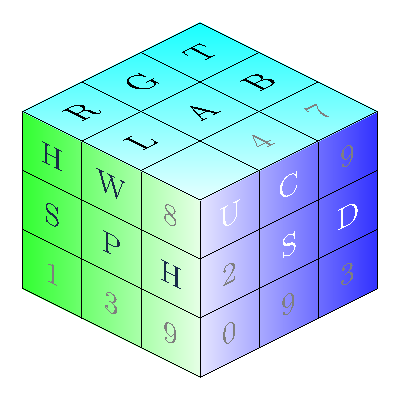
\includegraphics[width=3cm,valign=c]{sudoku.pdf}\\
\end{flushright}
\begin{flushleft} \LARGE } 
\posttitle{\par\end{flushleft}\vskip 0.5em} 
\predate{\begin{flushleft}\large} 
	\postdate{\par\end{flushleft}}
	\preauthor{\begin{flushleft}\large} 
	\postauthor{\par\end{flushleft}}
\rhead{\today}
\rfoot{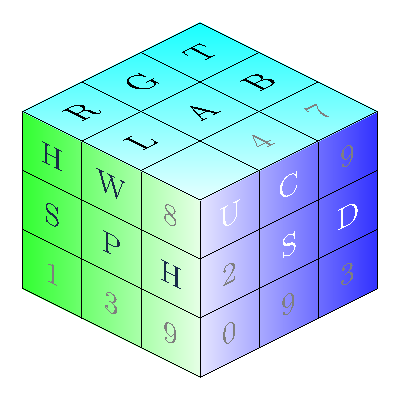
\includegraphics[width=1cm,valign=c]{sudoku.pdf}}





\rhead{ report}
\fancyhead[L]{\today} %put date in header
\fancyfoot[L]{c \currfilename} %put current file in footer
\setlength{\headheight}{13.59999pt}
\ifLuaTeX
  \usepackage{selnolig}  % disable illegal ligatures
\fi
\IfFileExists{bookmark.sty}{\usepackage{bookmark}}{\usepackage{hyperref}}
\IfFileExists{xurl.sty}{\usepackage{xurl}}{} % add URL line breaks if available
\urlstyle{same} % disable monospaced font for URLs
\hypersetup{
  pdfauthor={R.G. Thomas},
  hidelinks,
  pdfcreator={LaTeX via pandoc}}

\author{R.G. Thomas}
\date{2022-11-13}

\begin{document}

{
\setcounter{tocdepth}{2}
\tableofcontents
}
\thispagestyle{fancy}

\textbf{Variable type: factor}

\begin{tabular}{l|r|r|l|r|l}
\hline
skim\_variable & n\_missing & complete\_rate & ordered & n\_unique & top\_counts\\
\hline
Species & 0 & 1 & FALSE & 3 & set: 50, ver: 50, vir: 50\\
\hline
\end{tabular}

\textbf{Variable type: numeric}

\begin{tabular}{l|r|r|r|r|r|r|r|r|r}
\hline
skim\_variable & n\_missing & complete\_rate & mean & sd & p0 & p25 & p50 & p75 & p100\\
\hline
Sepal.Length & 0 & 1 & 5.8 & 0.83 & 4.3 & 5.1 & 5.8 & 6.4 & 7.9\\
\hline
Sepal.Width & 0 & 1 & 3.1 & 0.44 & 2.0 & 2.8 & 3.0 & 3.3 & 4.4\\
\hline
Petal.Length & 0 & 1 & 3.8 & 1.77 & 1.0 & 1.6 & 4.3 & 5.1 & 6.9\\
\hline
Petal.Width & 0 & 1 & 1.2 & 0.76 & 0.1 & 0.3 & 1.3 & 1.8 & 2.5\\
\hline
\end{tabular}

\hypertarget{introduction}{%
\section{Introduction}\label{introduction}}

\hypertarget{methods}{%
\section{Methods}\label{methods}}

\hypertarget{results}{%
\section{Results}\label{results}}

\hypertarget{code}{%
\section{Code}\label{code}}

\hypertarget{references}{%
\section{References}\label{references}}

Kuznetsova (2012) Sano et al. (1997) Thomas et al. (2000)

\hypertarget{refs}{}
\begin{CSLReferences}{1}{0}
\leavevmode\vadjust pre{\hypertarget{ref-KTIL5VTR}{}}%
Kuznetsova, OM. 2012. {``Considerations in the Paper by Proschan,
Brittain, and Kammerman Are Not an Argument Against Minimization. In
Response to Vance W Berger'Minimization: Not All It's.''} \emph{Clinical
Trials (London, England)}.
\url{http://www.ncbi.nlm.nih.gov/pubmed/22692807}.

\leavevmode\vadjust pre{\hypertarget{ref-W2FJ4NKV}{}}%
Sano, Mary, Christopher Ernesto, Ronald G. Thomas, Melville R. Klauber,
Kimberly Schafer, Michael Grundman, Peter Woodbury, et al. 1997. {``A
Controlled Trial of Selegiline, Alpha-Tocopherol, or Both as Treatment
for Alzheimer's Disease.''} \emph{New England Journal of Medicine} 336
(17): 1216--22. \url{https://doi.org/10.1056/NEJM199704243361704}.

\leavevmode\vadjust pre{\hypertarget{ref-CN948PZP}{}}%
Thomas, R.G., J.D. Berg, M. Sano, and L. Thal. 2000. {``Analysis of
Longitudinal Data in an Alzheimer's Disease Clinical Trial.''}
\emph{Statistics in Medicine} 19 (11-12).

\end{CSLReferences}

\end{document}
